\let\negmedspace\undefined
\let\negthickspace\undefined
\documentclass[journal]{IEEEtran}
\usepackage[a5paper, margin=10mm, onecolumn]{geometry}
%\usepackage{lmodern} % Ensure lmodern is loaded for pdflatex
\usepackage{tfrupee} % Include tfrupee package

\setlength{\headheight}{1cm} % Set the height of the header box
\setlength{\headsep}{0mm}     % Set the distance between the header box and the top of the text

\usepackage{gvv-book}
\usepackage{gvv}
\usepackage{cite}
\usepackage{amsmath,amssymb,amsfonts,amsthm}
\usepackage{algorithmic}
\usepackage{graphicx}
\usepackage{textcomp}
\usepackage{xcolor}
\usepackage{txfonts}
\usepackage{listings}
\usepackage{enumitem}
\usepackage{mathtools}
\usepackage{gensymb}
\usepackage{comment}
\usepackage[breaklinks=true]{hyperref}
\usepackage{tkz-euclide} 
\usepackage{listings}
% \usepackage{gvv}                                        
\def\inputGnumericTable{}                                 
\usepackage[latin1]{inputenc}                                
\usepackage{color}                                            
\usepackage{array}                                            
\usepackage{longtable}                                       
\usepackage{calc}                                             
\usepackage{multirow}                                         
\usepackage{hhline}                                           
\usepackage{ifthen}                                           
\usepackage{lscape}
\usepackage{circuitikz}
\tikzstyle{block} = [rectangle, draw, fill=blue!20, 
    text width=4em, text centered, rounded corners, minimum height=3em]
\tikzstyle{sum} = [draw, fill=blue!10, circle, minimum size=1cm, node distance=1.5cm]
\tikzstyle{input} = [coordinate]
\tikzstyle{output} = [coordinate]


\begin{document}

\bibliographystyle{IEEEtran}
\vspace{3cm}

\title{9-9.5-12}
\author{EE24BTECH11064 - Harshil Rathan}
 \maketitle
% \newpage
% \bigskip
{\let\newpage\relax\maketitle}

\renewcommand{\thefigure}{\theenumi}
\renewcommand{\thetable}{\theenumi}
\setlength{\intextsep}{10pt} % Space between text and floats


\numberwithin{equation}{enumi}
\numberwithin{figure}{enumi}
\renewcommand{\thetable}{\theenumi}

\textbf{Question}:\\
For the following differential equation, find the particular solution satisfying the given condition:\\
$x^2 dy + (xy+y^2) dx = 0 ; \text{ }y=1 \text{ }x=1 $\\
\solution \\
Let us solve the given equation theoretically and then verify the solution computationally
\begin{align}
    x^2 dy + \brak{xy +y^2} dx = 0 
\end{align}
\begin{align}
    \frac{dy}{dx}= - \frac{xy +y^2}{x^2}
    \label{0.2}
\end{align}
\begin{align}
    \frac{dy}{dx}= -\frac{y}{x} - (\frac{y}{x})^2
\end{align}
Let
\begin{align*}
    F\brak{x,y}=-\frac{(xy+y^2)}{x^2}
\end{align*}
\begin{align}
    F\brak{\lambda x,\lambda y}=\frac{[\lambda x \cdot \lambda y + (\lambda y)^2]}{(\lambda x)^2} = {\alpha}^0 \times F\brak{x,y}
\end{align}
Therefore, this is a homogeneous equation. We take the following substitution 
\begin{align}
    y = v x 
\end{align}
\begin{align}
    \frac{dy}{dx} = v + x \frac{dv}{dx}
\end{align}
\begin{align}
    x\frac{dv}{dx}=\frac{v-1}{v+1}-v
\end{align}
Substituting values of x and $\frac{dy}{dx}$ in \ref{0.2}
\begin{align}
    v + x \frac{dv}{dx} = - \frac{[x \cdot vx + (vx)^2]}{x^2} = -v -v^2
\end{align}
\begin{align}
    x\frac{dv}{dx} = -v(v+2)
\end{align}
\begin{align}
    \frac{dv}{v(v+2)} = - \frac{dx}{x}
\end{align}
\begin{align}
    \frac{1}{2} \frac{(v+2)-v}{v(v+2)} dv = - \frac{dx}{x}
\end{align}
\begin{align}
    \frac{1}{2} (\frac{1}{v} - \frac{1}{v+2}) dv = - \frac{dx}{x} 
\end{align}
Integrating on Both sides
\begin{align}
   \frac{1}{2}\int\frac{1}{v} \cdot dv + \frac{1}{2}\int\frac{1}{v+2}\cdot dv = -\int \frac{dx}{x}
\end{align}
\begin{align}
    \frac{1}{2}\log v + \frac{1}{2}\log (v+2) = - \log{x} + \log c
\end{align}
\begin{align}
    \frac{1}{2} \log (\frac{v}{v+2}) = \log \frac{C}{x}
\end{align}
\begin{align}
    \frac{v}{v+2} = (\frac{C}{x})^2
\end{align}
By substituting $v=\frac{y}{x}$ ,
\begin{align}
    \frac{x^2 y}{y+2x} =  C^2
    \label{0.17}
\end{align}
at x=1 and y =1 
\begin{align}
    C^2 = \frac{1}{3}
\end{align}
Substituting $C^2 = \frac{1}{3}$ in \ref{0.17} 
\begin{align}
    \frac{x^2y}{y+2x} = \frac{1}{3}
\end{align}
\begin{align}
    y+2x = 3x^2y
\end{align}
Now lets verify the solution computationally from the definition of $\frac{dy}{dx}$
\begin{align}
    y_{n+1}= y_{n} + \frac{dy}{dx} \cdot h
    \label{0.21}
\end{align}
From the differential equation given,
\begin{align}
    \frac{dy}{dx} = \frac{y_n - x_n}{y_n + x_n}
    \label{0.22}
\end{align}
Substituting \ref{0.22} in \ref{0.21}
\begin{align}
    y_{n+1} = y_n + \brak{\frac{y_n - x_n}{y_n + x_n}} \cdot h 
\end{align}
\begin{figure}
    \centering
    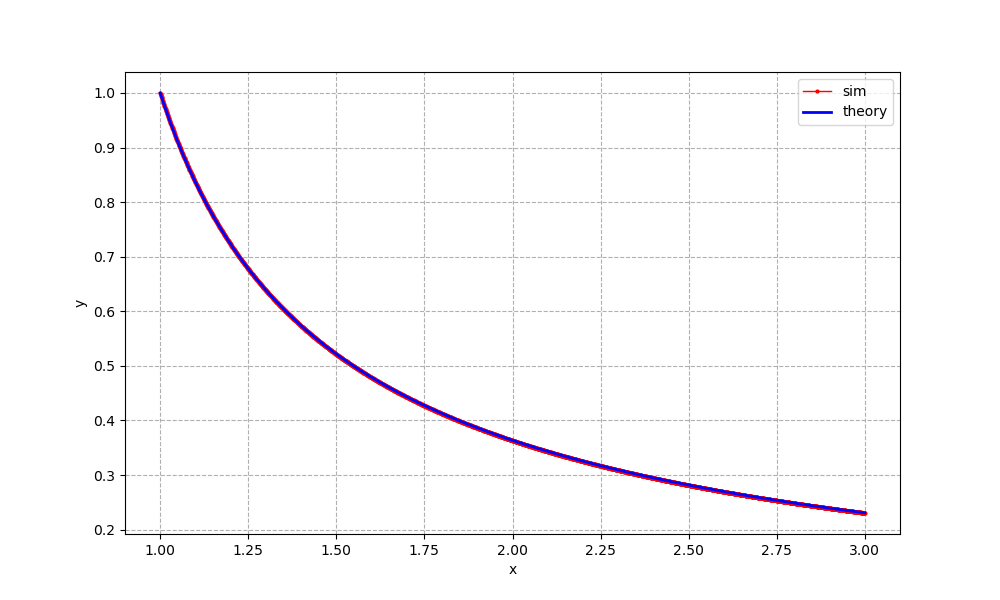
\includegraphics[width=\columnwidth]{figs/Figure_1.png}
\end{figure}
The comparison between theoretical and simulation curves is shown in the figure, we can clearly see that both the curves are coincides which verifies our solution
\end{document}



